\chapter{Установка multicorda}

\section{Тулчейн для разработки и отладки}

В качестве ассемблера используется Flat Assembler (fasm). Он был выбран за кроссплатформенность, возможность сборки бинарных файлов без заголовков ELF/PE и удобные макросы.

В качестве виртуальной машины и отладчика используется Bochs. Он позволяет отлаживать код с момента передачи управления BIOS, а также изучать полное состояние процессора и памяти в любой момент выполнения программы.

\subsection{Установка fasm}

Последнюю версию fasm можно скачать по ссылке\\ \verb|https://flatassembler.net/download.php|. Для запуска multicorda необходим fasm 1.73 или новее. 

fasm распространяется в виде zip-архива, для установки его нужно разархивировать в любую папку. Версия для Windows включает в себя небольшую IDE (fasmw.exe), в которой можно редактировать код и сразу его ассемблировать.

\subsection{Установка Bochs}

Последнюю версию Bochs (2.7) можно скачать по ссылке\\ \verb|https://sourceforge.net/projects/bochs/files/bochs/2.7/|. После установки на Windows файлы \verb|.bxrc| будут автоматически открываться в Bochs. Для запуска отладчика необходимо найти в папке установки файл \verb|bochsdbg.exe|. 

\section{Сборка multicorda}

Для сборки multicorda необходимо открыть файл \verb|main.asm| в fasmw и нажать:

\begin{center}
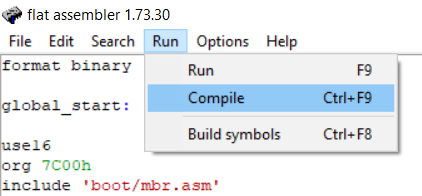
\includegraphics{pictures/2-compiling}
\end{center}

После этого в папке с исходным кодом будет создан файл \verb|main.bin|, являющийся образом дискеты для запуска multicorda.

\section{Запуск multicorda}

Примеры конфигурационных файлов для Bochs и Bochsdbg приложены к документации. Для простого запуска multicorda достаточно открыть файл \verb|.bxrc|, после чего запустится Bochs:

\begin{center}
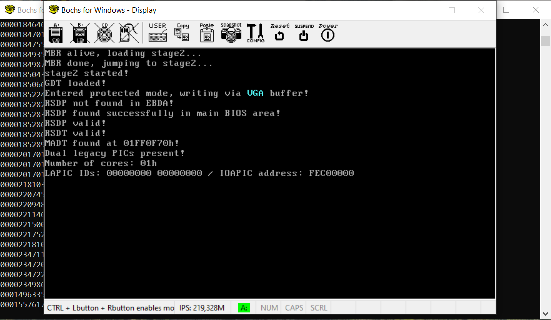
\includegraphics{pictures/2-simple-launch}
\end{center}

Для запуска дебаггера нужно запустить \verb|bochsdbg.exe| и выбрать конфигурационный файл через Load, после чего нажать Start. После этого ВМ будет ожидать запуска симуляции путем нажатия на кнопку Continue:

\begin{center}
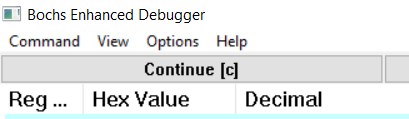
\includegraphics{pictures/2-start-debugging}
\end{center}

Также возможно использовать для запуска и отладки связку QEMU+GDB, однако это выходит за пределы данного руководства.